\documentclass[tikz,border=12pt]{standalone}
\usepackage[T1]{fontenc}
\usepackage{mathpazo}
\usepackage{amsmath,amssymb}
\usetikzlibrary{arrows.meta, positioning, calc, decorations.pathreplacing}

\definecolor{stblue}{HTML}{7B97AD}
\definecolor{rwgold}{HTML}{B8995E}
\definecolor{sage}{HTML}{7A9A7E}
\definecolor{dkbrown}{HTML}{3D3530}
\definecolor{wmgray}{HTML}{7B7067}
\definecolor{cream}{HTML}{F9F6F0}
\definecolor{border}{HTML}{D4C9B8}
\definecolor{terracotta}{HTML}{C47A6A}
\definecolor{lavender}{HTML}{907EA0}

\begin{document}
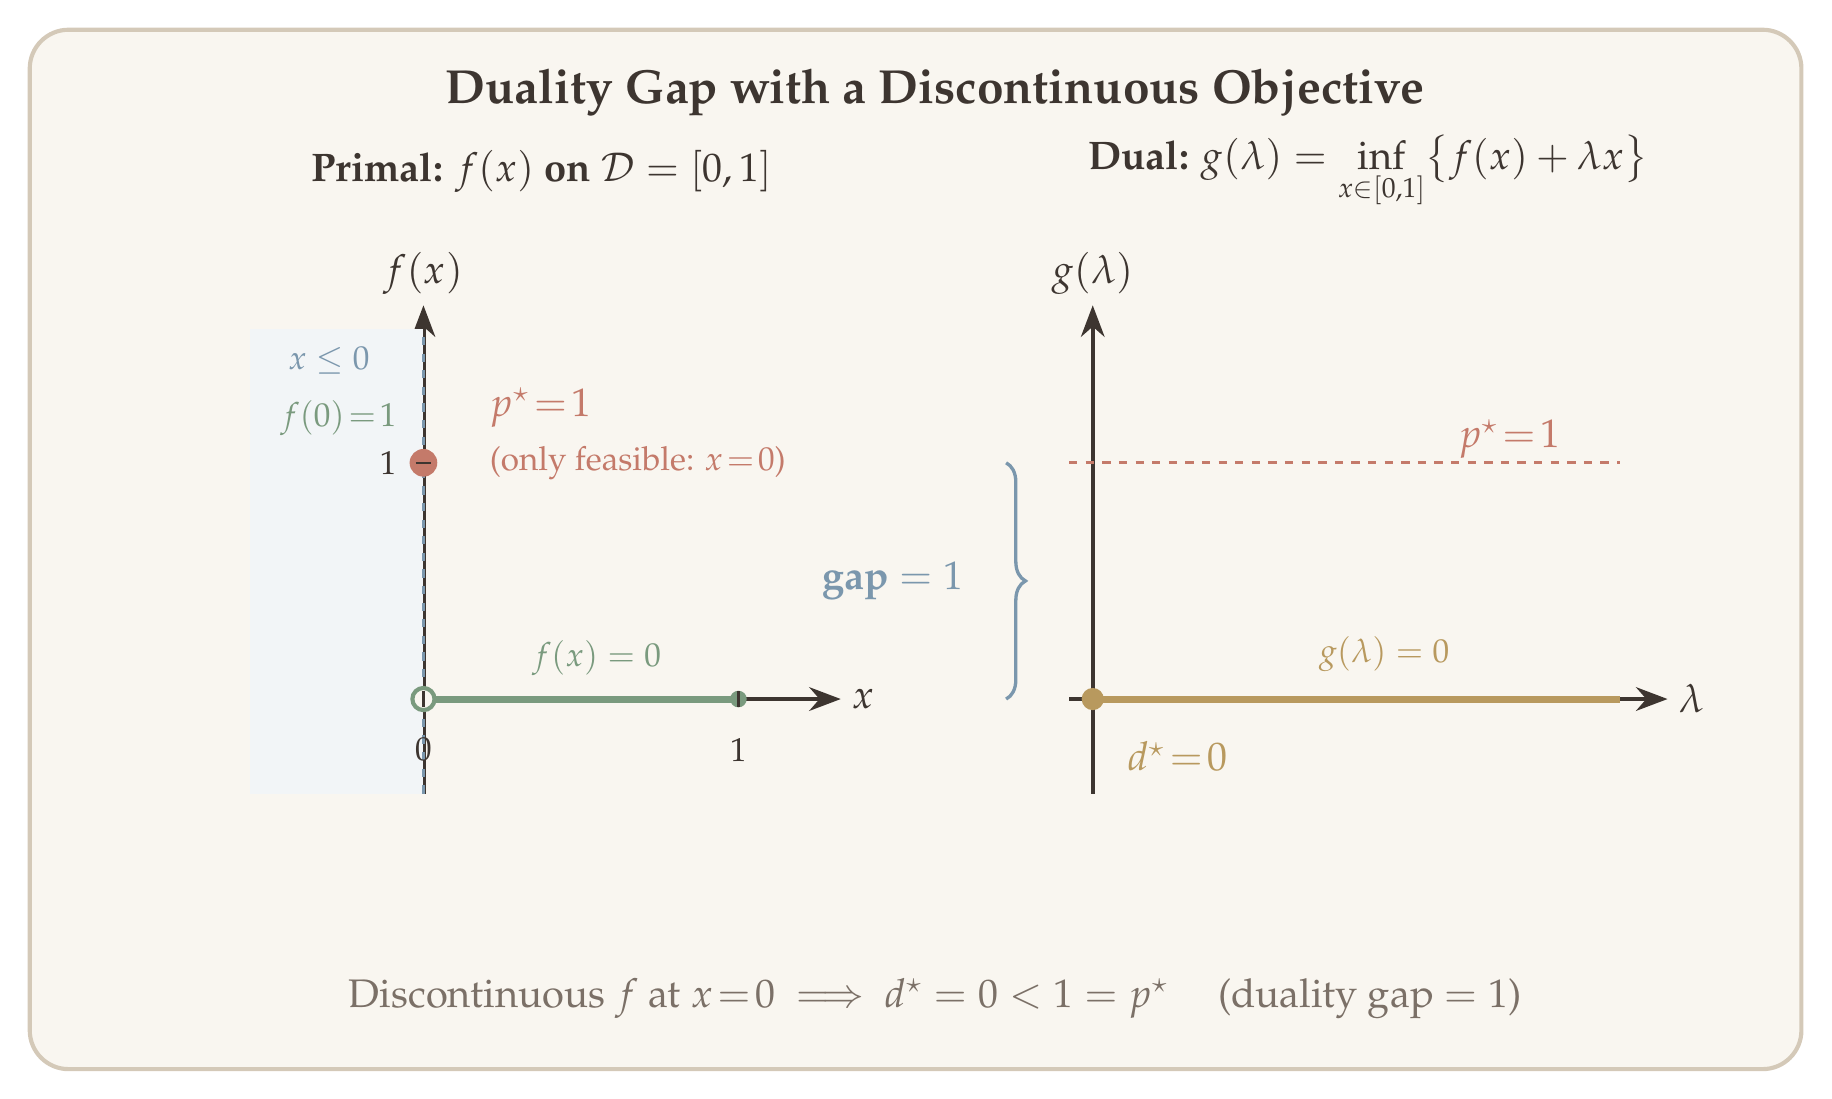
\begin{tikzpicture}[>={Stealth[length=4mm, width=3mm]}, line width=1.5pt]

% Background
\fill[cream, rounded corners=14pt] (-2.5,-3.2) rectangle (20,10);
\draw[border, line width=1.5pt, rounded corners=14pt] (-2.5,-3.2) rectangle (20,10);

% Title
\node[font=\LARGE\bfseries, text=dkbrown, align=center] at (9,9.2)
  {Duality Gap with a Discontinuous Objective};

% ================================================================
% LEFT PANEL
% ================================================================
\begin{scope}[shift={(0,0)}]

% Panel label — very high, well above everything
\node[font=\Large\bfseries, text=dkbrown] at (4,8.2)
  {Primal: $f(x)$ on $\mathcal{D}=[0,1]$};

% Coordinate mapping:
%   x=0 at tikzX=2.5, scale 4.0 per unit
%   f=0 at tikzY=1.5, f=1 at tikzY=4.5 (scale 3.0)

% Axes
\draw[->, dkbrown, line width=1.5pt] (0.3,1.5) -- (7.8,1.5)
  node[right, font=\Large, text=dkbrown] {$x$};
\draw[->, dkbrown, line width=1.5pt] (2.5,0.3) -- (2.5,6.5)
  node[above, font=\Large, text=dkbrown] {$f(x)$};

% Feasible region x <= 0 shading — to the left of x=0
\fill[stblue!10] (0.3,0.3) rectangle (2.5,6.2);
\node[font=\large, text=stblue] at (1.3,5.8) {$x \le 0$};

% Dashed line at x=0
\draw[stblue, dashed, line width=1pt] (2.5,0.3) -- (2.5,6.2);

% Step function: f(0) = 1, f(x) = 0 for x in (0,1]
% Open dot at (0, 0): tikz (2.5, 1.5)
\draw[sage, line width=1.5pt, fill=cream] (2.5,1.5) circle (4pt);

% Horizontal line f=0 from x=0+ to x=1: tikz (2.65, 1.5) to (6.5, 1.5)
\draw[sage, line width=2.5pt] (2.65,1.5) -- (6.5,1.5);

% Endpoint at x=1
\fill[sage] (6.5,1.5) circle (3pt);

% Solid dot at (0, 1): tikz (2.5, 4.5)
\fill[terracotta] (2.5,4.5) circle (5pt);

% p* label — offset to the right and up, clear of the open dot below
\node[font=\Large\bfseries, text=terracotta, anchor=west] at (3.2,5.2)
  {$p^\star\!=\!1$};
\node[font=\large, text=terracotta, anchor=west] at (3.2,4.5)
  {(only feasible: $x\!=\!0$)};

% x-axis ticks
\draw[dkbrown, line width=0.8pt] (2.5,1.4) -- (2.5,1.6);
\node[font=\large, text=dkbrown, below] at (2.5,1.15) {$0$};
\draw[dkbrown, line width=0.8pt] (6.5,1.4) -- (6.5,1.6);
\node[font=\large, text=dkbrown, below] at (6.5,1.15) {$1$};

% f-axis tick at f=1
\draw[dkbrown, line width=0.8pt] (2.4,4.5) -- (2.6,4.5);
\node[font=\large, text=dkbrown, anchor=east] at (2.3,4.5) {$1$};

% Function labels — well separated
\node[font=\large, text=sage, above] at (4.7,1.65) {$f(x)=0$};
\node[font=\large, text=sage, anchor=south east] at (2.3,4.7) {$f(0)\!=\!1$};

\end{scope}

% ================================================================
% RIGHT PANEL
% ================================================================
\begin{scope}[shift={(10.5,0)}]

% Panel label
\node[font=\Large\bfseries, text=dkbrown] at (4,8.2)
  {Dual: $g(\lambda) = \displaystyle\inf_{x \in [0,1]}\bigl\{f(x)+\lambda x\bigr\}$};

% Same vertical scale: g=0 at tikzY=1.5, g=1 at tikzY=4.5

% Axes
\draw[->, dkbrown, line width=1.5pt] (0.2,1.5) -- (7.8,1.5)
  node[right, font=\Large, text=dkbrown] {$\lambda$};
\draw[->, dkbrown, line width=1.5pt] (0.5,0.3) -- (0.5,6.5)
  node[above, font=\Large, text=dkbrown] {$g(\lambda)$};

% g(lambda) = 0 flat line
\draw[rwgold, line width=2.5pt] (0.5,1.5) -- (7.2,1.5);

% Mark d* = 0
\fill[rwgold] (0.5,1.5) circle (4pt);
\node[font=\Large\bfseries, text=rwgold, anchor=north west] at (0.8,1.1)
  {$d^\star\!=\!0$};

% g(lambda) label
\node[font=\large, text=rwgold, above] at (4.2,1.7) {$g(\lambda)=0$};

% p* level
\draw[terracotta, dashed, line width=1pt] (0.2,4.5) -- (7.2,4.5);
\node[font=\Large\bfseries, text=terracotta, anchor=west] at (5,4.8)
  {$p^\star\!=\!1$};

% Brace for duality gap — moved further left for clearance
\draw[decorate, decoration={brace, amplitude=7pt, mirror}, stblue, line width=1.2pt]
  (-0.6,1.5) -- (-0.6,4.5);
\node[font=\Large\bfseries, text=stblue, anchor=east] at (-1.0,3.0)
  {gap $=1$};

\end{scope}

% Bottom annotation
\node[font=\Large, text=wmgray, align=center] at (9,-2.3)
  {Discontinuous $f$ at $x\!=\!0$ $\implies$ $d^\star = 0 < 1 = p^\star$ \quad (duality gap $= 1$)};

\end{tikzpicture}
\end{document}
